\documentclass[border=4pt]{standalone}
\usepackage[usenames,dvipsnames,svgnames]{xcolor}
\usepackage{pgfgantt}
\usetikzlibrary{positioning}
\usetikzlibrary{backgrounds}
\newcounter{myWeekNum}
\stepcounter{myWeekNum}
%
\newcommand{\myWeek}{\themyWeekNum
    \stepcounter{myWeekNum}
    \ifnum\themyWeekNum=53
         \setcounter{myWeekNum}{1}
    \else\fi
}

\tikzstyle{unassigned}=[] 
\tikzstyle{name_0}=[fill=JungleGreen]
\tikzstyle{name_1}=[fill=RedOrange]
\tikzstyle{name_2}=[fill=Dandelion]

\begin{document}


    \setcounter{myWeekNum}{24}
    \ganttset{calendar week text={\myWeek{}}}
    \begin{ganttchart}[
        x unit=0.6125cm,
    	y unit chart=0.5cm,
    	hgrid=true,
    	vgrid=true,
    	time slot format=isodate
    ]{2021-06-20}{2021-08-12}

    \gantttitlecalendar{year, month=name, week}
    

        \\\ganttgroup{Task Group 1}
        {2021-06-20}{2021-06-30}
        

            \\\ganttbar[bar/.append style=name_0]
            {Task 1}
            {2021-06-20}{2021-06-26}
            

            \\\ganttbar[bar/.append style=name_1]
            {Task 3}
            {2021-06-20}{2021-06-27}
            

            \\\ganttbar[bar/.append style=name_0]
            {Task 2}
            {2021-06-27}{2021-06-30}
            

        \\
        

        \\\ganttgroup{Task Group 2}
        {2021-06-28}{2021-07-15}
        

            \\\ganttbar[bar/.append style=name_1]
            {Task 4}
            {2021-06-28}{2021-07-11}
            

            \\\ganttbar[bar/.append style=name_0]
            {Task 5}
            {2021-07-01}{2021-07-15}
            

        \\
        

        \\\ganttgroup{Task Group 3}
        {2021-06-30}{2021-07-11}
        

            \\\ganttbar[bar/.append style=name_2]
            {Task 6}
            {2021-06-30}{2021-07-05}
            

            \\\ganttbar[bar/.append style=unassigned]
            {Task 7}
            {2021-06-30}{2021-07-11}
            

        \\
        

        \\\ganttgroup{Task Group 4}
        {2021-07-06}{2021-07-25}
        

            \\\ganttbar[bar/.append style=name_2]
            {Task 8}
            {2021-07-06}{2021-07-13}
            

            \\\ganttbar[bar/.append style=unassigned]
            {Task 9}
            {2021-07-12}{2021-07-25}
            

            \\\ganttbar[bar/.append style=name_2]
            {Task 10}
            {2021-07-14}{2021-07-25}
            

            \\\ganttbar[bar/.append style=name_0]
            {Task 11}
            {2021-07-16}{2021-07-25}
            

        \\
        

        \\\ganttgroup{Task Group 5}
        {2021-07-16}{2021-08-12}
        

            \\\ganttbar[bar/.append style=name_1]
            {Task 12}
            {2021-07-16}{2021-07-25}
            

            \\\ganttbar[bar/.append style=name_2]
            {Task 13}
            {2021-07-26}{2021-08-04}
            

            \\\ganttbar[bar/.append style=unassigned]
            {Task 14}
            {2021-08-05}{2021-08-12}
            

        \\
        

    \end{ganttchart}
    

    \hspace{0.125in}
    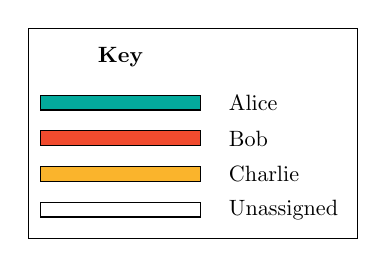
\begin{tikzpicture}[framed,scale=0.8,every node/.style={transform shape}]
    \node (kh) [] {\textbf{Key}};
    
\node (b0) [below=0.125in of kh, name_0, rectangle,draw,minimum width=1in]{};
\node (b1) [below=0.125in of b0, name_1, rectangle,draw,minimum width=1in]{};
\node (b2) [below=0.125in of b1, name_2, rectangle,draw,minimum width=1in]{};
\node (b3) [below=0.125in of b2, unassigned, rectangle,draw,minimum width=1in]{};
\node (l0) [right=0.125in of b0]{Alice};
\node (l1) [right=0.125in of b1]{Bob};
\node (l2) [right=0.125in of b2]{Charlie};
\node (l3) [right=0.125in of b3]{Unassigned};
\end{tikzpicture}

\end{document}

